\documentclass{beamer}
\usepackage{animate}
\usepackage{tikz}
\usepackage{svg}
\usetheme{metropolis}
\begin{document}

\begin{frame}{\small{What is calibration in Astronomy?}}
\begin{figure}[h]
  \centering
  \includesvg[width=0.8\textwidth]{whatiscal.svg}
\end{figure}
    \tiny{Co-authors: Harry Bevins, Will Handley, Eloy de Lera Acedo, Jiacong Zhu, Kaan Artuc, Daniel Molnar}
  \end{frame}


\begin{frame}{\small{How to calibrate?}}
\begin{figure}[h]
  \centering
  \includesvg[width=0.8\textwidth]{howtocal.svg}
\end{figure}
    \tiny{Co-authors: Harry Bevins, Will Handley, Eloy de Lera Acedo, Jiacong Zhu, Kaan Artuc, Daniel Molnar}
  \end{frame}


\begin{frame}{\small{Why is machine learning helpful?}}
\begin{figure}[h]
  \centering
  \includesvg[width=0.7\textwidth]{mlcal.svg}
\end{figure}
    \tiny{Co-authors: Harry Bevins, Will Handley, Eloy de Lera Acedo, Jiacong Zhu, Kaan Artuc, Daniel Molnar}
  \end{frame}

\begin{frame}{\small{Machine learning for radiometer calibration in global 21cm cosmology}}
  \begin{figure}
    \centering
    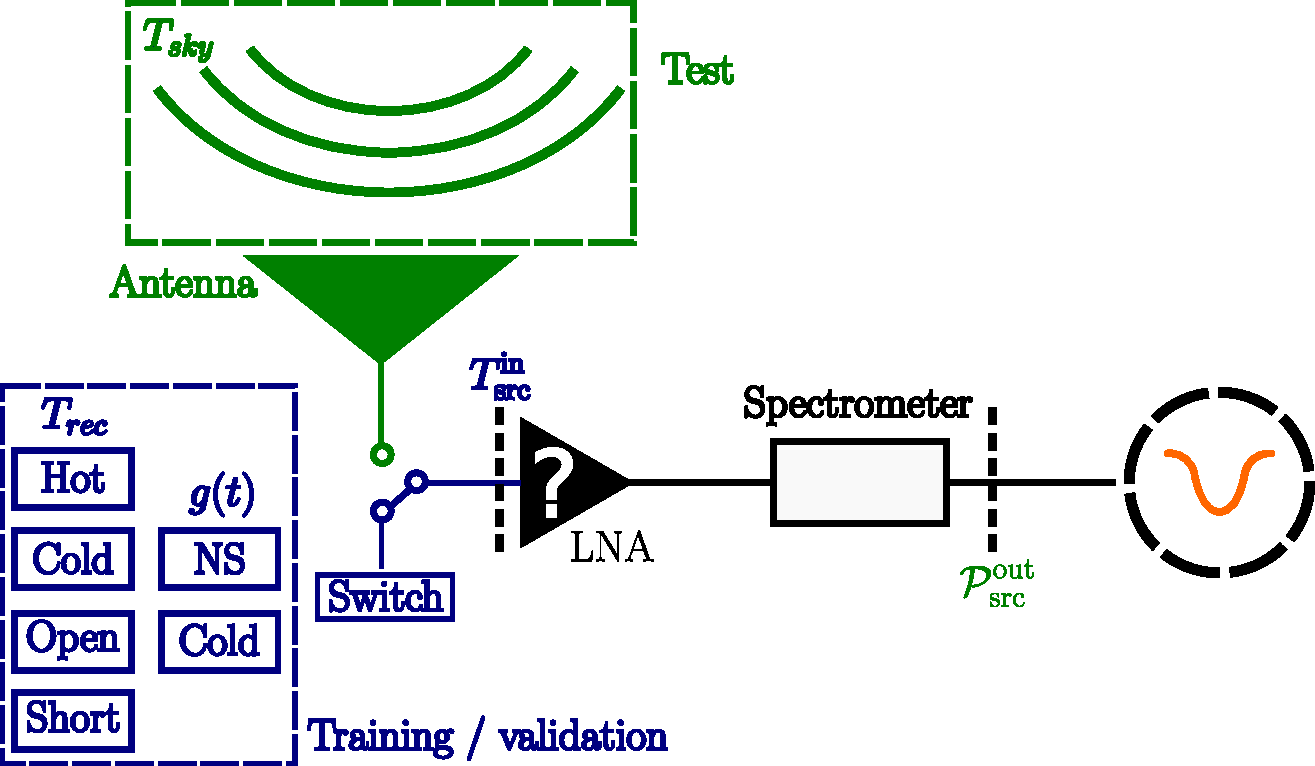
\includegraphics[width=1.05\textwidth]{instrument.pdf}
  \end{figure}
    \vspace{0.3cm}
    \tiny{Co-authors: Harry Bevins, Will Handley, Eloy de Lera Acedo, Jiacong Zhu, Kaan Artuc, Daniel Molnar}
  \end{frame}

  \begin{frame}{\small{Machine learning for radiometer calibration in global 21cm cosmology}}
    \begin{figure}
    \centering
    \includesvg[width=0.9\textwidth]{nn.svg}
  \end{figure}

    \tiny{Co-authors: Harry Bevins, Will Handley, Eloy de Lera Acedo, Jiacong Zhu, Kaan Artuc, Daniel Molnar}

  \end{frame}

  \begin{frame}{\small{Machine learning for radiometer calibration in global 21cm cosmology}}
    \begin{figure}
      \centering
      \includesvg[width=\textwidth]{results.svg}
    \end{figure}
    \begin{figure}
      \centering
      \includegraphics[width=0.8\textwidth]{header.png}
    \end{figure}
    \vspace{0.3cm}
    \tiny{Co-authors: Harry Bevins, Will Handley, Eloy de Lera Acedo, Jiacong Zhu, Kaan Artuc, Daniel Molnar}
  \end{frame}
\end{document}
